\section{Radiodifusión en FM}
\label{sec:fm}

\subsection{Modulación FM}
En la modulación de frecuencia, la frecuencia instantánea de la portadora se desvía en proporción a la señal modulante. Para un tono de frecuencia $f_m$ que produce una desviación máxima $\Delta f$, el índice de modulación es $\beta = \Delta f / f_m$ y la señal se desarrolla en funciones de Bessel de primera especie ($J_n(\beta)$) \cite{haykin}:
\begin{equation}
    v_{FM} = E_c \cos\left[2\pi f_c t + \beta \sin(2\pi f_m t)\right]
    = E_c \sum_{n=-\infty}^{\infty} J_n(\beta) \cos\left[2\pi (f_c + n f_m) t\right]
    \label{eq:fm}
\end{equation}

El espectro tiene infinitas componentes separadas $f_m$ entre sí, con amplitud $E_c J_n(\beta)$. Cada coeficiente da la amplitud relativa de la componente en $f_c + n f_m$: $J_0(\beta)$ corresponde a la portadora y $J_n(\beta)$, con $n \neq 0$, al par de bandas laterales de orden $n$. Como $J_{-n}(\beta) = (-1)^n J_n(\beta)$, las bandas laterales de un mismo orden tienen igual amplitud, y difieren sólo en el signo cuando $n$ es impar. Además, se cumple
\begin{equation}
    J_0^2(\beta) + 2 \sum_{n=1}^{\infty} J_n^2(\beta) = 1
\end{equation}
lo que indica que la potencia total es constante: la modulación sólo la redistribuye entre la portadora y las bandas laterales \cite{haykin}.

El número de componentes significativas crece con $\beta$. Con $\beta \ll 1$ (FM de banda angosta) sólo son apreciables $J_0 \approx 1$ y $J_1 \approx \beta/2$, y el espectro se parece al de una AM, con un par de bandas laterales. A medida que $\beta$ aumenta, la potencia se reparte en más pares, del orden de $\beta + 1$, por lo que casi toda la potencia queda en el ancho de banda que da la regla de Carson:

\begin{equation}
    B_T \approx 2 \left(\Delta f + f_m\right)
    \label{eq:carson}
\end{equation}

En la radiodifusión en FM la desviación máxima es de $\pm 75 \, [kHz]$ \cite{itu_bs450}. La señal que modula la portadora no es directamente el audio, sino la señal múltiplex estéreo, que agrupa en banda base las componentes de la \autoref{tab:fm_multiplex} (\autoref{fig:fm_multiplex}). El esquema es compatible con los receptores monofónicos, que sólo aprovechan la parte de $30 \, [Hz]$ a $15 \, [kHz]$, mientras que un receptor estéreo recupera ambos canales como $L = M + S$ y $R = M - S$.

\begin{table}[H]
    \centering
    \caption{Componentes de la señal múltiplex estéreo \cite{itu_bs450, itu_bs643}.}
    \label{tab:fm_multiplex}
    \renewcommand{\arraystretch}{1.3}
    \begin{tabular}{l l >{\raggedright\arraybackslash}p{7.6cm}}
        \toprule
        \textbf{Frecuencia} & \textbf{Componente} & \textbf{Función} \\
        \midrule
        $30 \, [Hz]$ a $15 \, [kHz]$ & $M = (L+R)/2$ & Suma de ambos canales: es la señal que reproduce un receptor monofónico. \\
        $19 \, [kHz]$ & Tono piloto & Referencia con la que el receptor regenera la subportadora de $38 \, [kHz]$, su segunda armónica. \\
        $23$ a $53 \, [kHz]$ & $S = (L-R)/2$ & Diferencia entre canales, en doble banda lateral con la subportadora de $38 \, [kHz]$ suprimida. \\
        $57 \, [kHz]$ & RDS (opcional) & Datos de identificación de la emisora y del programa, a $1187{,}5 \, [bit/s]$, sobre una subportadora suprimida enganchada a la tercera armónica del piloto. \\
        \bottomrule
    \end{tabular}
\end{table}

Las componentes se reparten la desviación máxima. Según la Recomendación UIT-R BS.450, $M$ y $S$ pueden alcanzar cada una el $90 \, $\% de la desviación, pero en condiciones distintas: con $L = R$ toda la señal está en $M$, y con $L = -R$ toda está en $S$. El tono piloto ocupa entre el $8$ y el $10 \, $\%, y el conjunto de las subportadoras adicionales, entre $53$ y $76 \, [kHz]$, no puede superar el $10 \, $\% \cite{itu_bs450}. Para el RDS se recomienda una desviación nominal de $\pm 2 \, [kHz]$ \cite{itu_bs643}.

Con la regla de Carson, la señal monofónica ocupa $2(75 + 15) = 180 \, [kHz]$ y la estéreo $2(75 + 53) = 256 \, [kHz]$. Este último valor es mayor que la separación de $200 \, [kHz]$ entre canales, porque la regla es conservadora: la desviación pico sólo se alcanza en los momentos de mayor nivel del programa, y las componentes de mayor frecuencia de la múltiplex no usan toda la desviación.

\begin{figure}[H]
    \centering
    \begin{tikzpicture}[x=0.165cm, y=0.05cm, font=\small]
        % Ejes
        \draw[-{Stealth[length=2mm]}] (0,0) -- (80,0) node[right] {$f \, [kHz]$};
        \draw[-{Stealth[length=2mm]}] (0,0) -- (0,108) node[above] {\% de $\Delta f_{max}$};
        \foreach \x in {0,15,19,23,38,53,57,76}
            \draw (\x,0) -- (\x,-1.5) node[below=1pt, font=\scriptsize] {\x};
        \foreach \y in {10,90,100}
            \draw (0,\y) -- (-1,\y) node[left, font=\scriptsize] {\y};
        \draw[densely dotted, gray] (0,100) -- (78,100);
        % M = (L+R)/2
        \draw[thick, blue!70!black, fill=blue!10] (0.03,0) -- (0.03,90) -- (15,90) -- (15,0);
        \node[blue!70!black, align=center] at (7.5,55) {$(L+R)/2$};
        % Piloto
        \draw[very thick, red!75!black] (19,0) -- (19,10);
        \node[red!75!black, above] at (19,10) {Piloto};
        % S = (L-R)/2, DBL con portadora suprimida en 38 kHz
        \draw[thick, green!45!black, fill=green!10] (23,0) -- (23,90) -- (37.97,90) -- (37.97,0);
        \draw[thick, green!45!black, fill=green!10] (38.03,0) -- (38.03,90) -- (53,90) -- (53,0);
        \node[green!45!black, align=center] at (30.5,45) {BLI};
        \node[green!45!black, align=center] at (45.5,45) {BLS};
        \node[green!45!black, fill=green!10, inner sep=1pt] at (38,76) {$(L-R)/2$, DBL-PS};
        \draw[dashed, green!45!black] (38,0) -- (38,90);
        \node[green!45!black, font=\scriptsize, fill=white, inner sep=1pt] at (38,22) {38 kHz};
        % RDS
        \draw[thick, orange!80!black, fill=orange!15] (55,0) -- (55,4) -- (59,4) -- (59,0);
        \node[orange!80!black, above] at (57,4) {RDS};
        % Zona de subportadoras adicionales
        \draw[decorate, decoration={brace, amplitude=4pt, mirror}] (53,-9) -- (76,-9)
            node[midway, below=5pt, font=\scriptsize, align=center] {Subportadoras adicionales\\($53$ a $76 \, [kHz]$, $\leq 10 \, $\%)};
    \end{tikzpicture}
    \caption{Espectro de la señal múltiplex estéreo en banda base (esquema propio basado en \cite{itu_bs450, itu_bs643}). La altura de cada componente indica su amplitud máxima como porcentaje de la desviación máxima; $M$ y $S$ alcanzan el $90 \, $\% en condiciones distintas, por lo que no lo hacen al mismo tiempo.}
    \label{fig:fm_multiplex}
\end{figure}

\subsection{Mediciones}

\subsubsection*{Exploración de la banda}
Se exploró la banda de $88$ a $108 \, [MHz]$ con un RBW de $9 \, [kHz]$ (\autoref{fig:fm_completa}). Sobre un piso de ruido de unos $-96 \, [dBm]$ se distinguen alrededor de una docena de emisoras, con niveles entre unos $-90$ y $-65 \, [dBm]$. Con un \textit{span} de $20 \, [MHz]$ cada emisora aparece como una línea, porque su ancho, del orden de $200 \, [kHz]$, ocupa apenas un punto de la traza.

\begin{figure}[H]
    \centering
    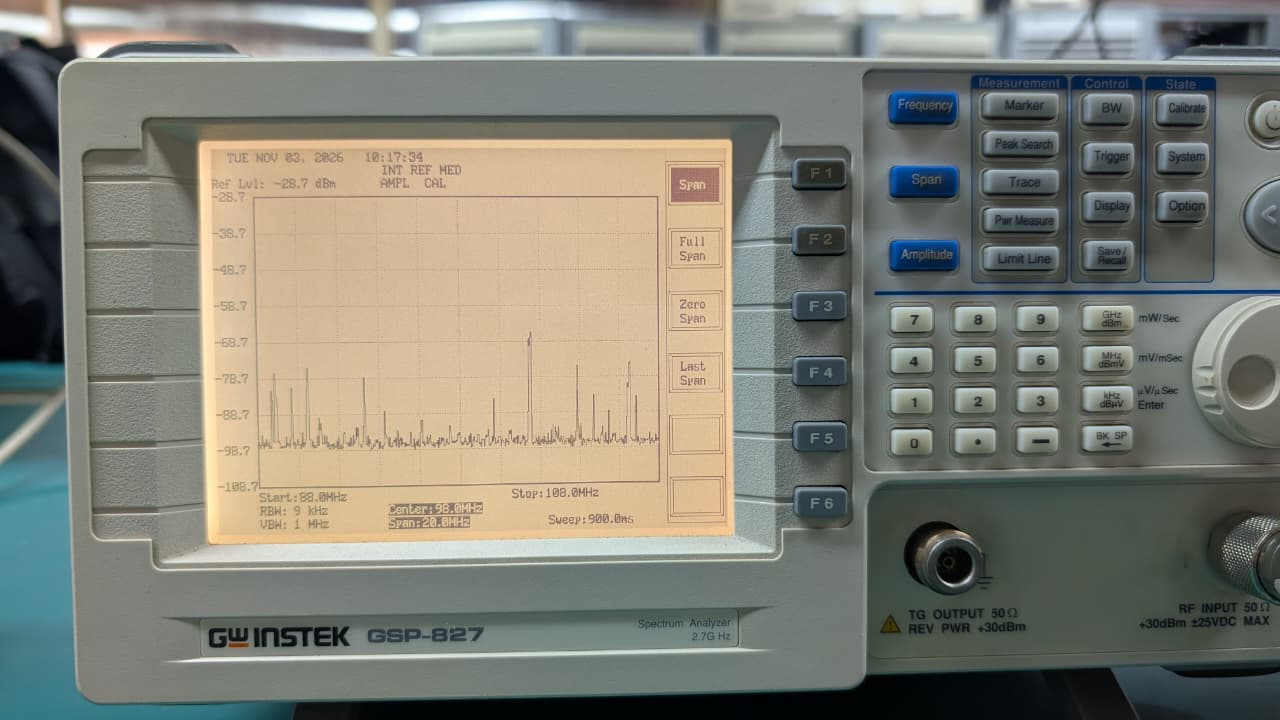
\includegraphics[width=0.8\textwidth]{fm_completa.png}
    \caption{Exploración de la banda de radiodifusión en FM.}
    \label{fig:fm_completa}
\end{figure}

\begin{table}[H]
    \centering
    \caption{Configuración del analizador y resultados en la banda de FM.}
    \label{tab:fm_resultados}
    \begin{tabular}{p{8.5cm} >{\raggedright\arraybackslash}p{5.8cm}}
        \toprule
        \textbf{Parámetro} & \textbf{Valor} \\
        \midrule
        Frecuencias de inicio y fin & $88$ a $108 \, [MHz]$ \\
        Frecuencia central & $98 \, [MHz]$ \\
        \textit{Span} & $20 \, [MHz]$ \\
        Nivel de referencia & $-28{,}7 \, [dBm]$ \\
        RBW / VBW & $9 \, [kHz]$ / $1 \, [MHz]$ \\
        \midrule
        \textbf{Emisora 1} \\
        \midrule
        Frecuencia de la portadora & $88{,}9 \, [MHz]$ \\
        Emisora identificada & No confirmada \\
        \textit{Span} & $600 \, [kHz]$ \\
        Nivel de referencia & $-60 \, [dBm]$ \\
        RBW / VBW & $3 \, [kHz]$ / $100 \, [kHz]$ \\
        Nivel de la portadora & $\approx -70 \, [dBm]$ (máximo de la envolvente) \\
        \midrule
        \textbf{Emisora 2} \\
        \midrule
        Frecuencia de la portadora & $102{,}3 \, [MHz]$ \\
        Emisora identificada & No confirmada \\
        \textit{Span} & $200 \, [kHz]$ \\
        Nivel de referencia & $-90 \, [dBm]$ \\
        RBW / VBW & $300 \, [Hz]$ / $30 \, [kHz]$ \\
        Nivel de la portadora & $\approx -92 \, [dBm]$ (componente máxima) \\
        \bottomrule
    \end{tabular}
\end{table}

\begin{figure}[H]
    \centering
    \begin{subfigure}[b]{0.485\textwidth}
        \centering
        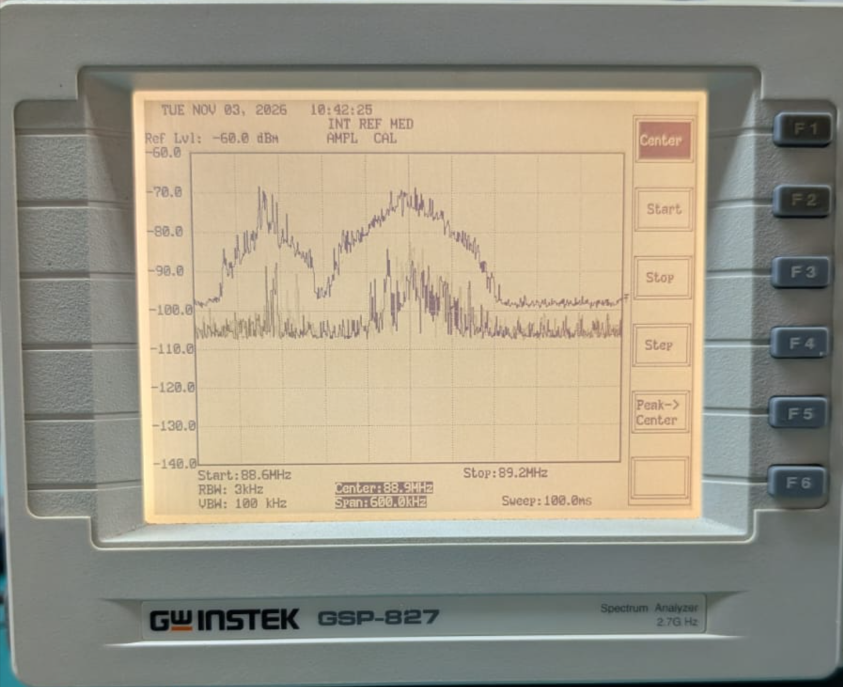
\includegraphics[width=\linewidth]{fm_emisora1.png}
        \caption{Emisora 1 ($88{,}9 \, [MHz]$).}
        \label{fig:fm_emisora1}
    \end{subfigure}
    \hfill
    \begin{subfigure}[b]{0.5\textwidth}
        \centering
        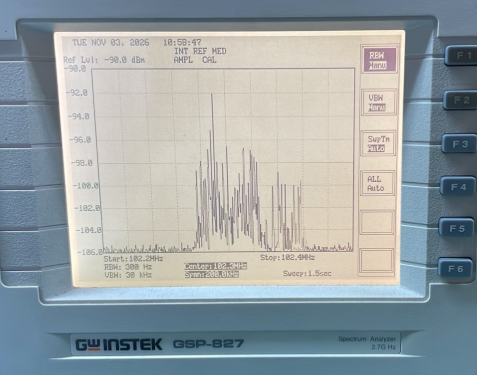
\includegraphics[width=\linewidth]{fm_emisora2.png}
        \caption{Emisora 2 ($102{,}3 \, [MHz]$).}
        \label{fig:fm_emisora2}
    \end{subfigure}
    \caption{Espectro de las emisoras de FM analizadas.}    \label{fig:fm_emisoras}
\end{figure}

Ninguna de las dos emisoras pudo confirmarse en el listado oficial de ENACOM. Según listados de emisoras no oficiales, la de $88{,}9 \, [MHz]$ correspondería a Pobre Johnny 88,9 FM y la de $102{,}3 \, [MHz]$ a CBA24 102,3 FM, ambas de la ciudad de Córdoba \cite{tuningaradio}.

\subsection{Análisis}

\subsubsection*{Ancho de banda ocupado}
Con una señal de programa, el espectro de FM no muestra una portadora fija y bandas laterales separadas, como con un tono: la energía se mueve dentro de un ``bloque'' de ancho variable alrededor de $f_c$. Por eso el ancho de banda se estimó sobre la envolvente en retención de máximos de la Emisora 1 (\autoref{fig:fm_emisora1}), entre los puntos que caen $26 \, [dB]$ por debajo del máximo \cite{itu_sm328}. Con el máximo en unos $-70 \, [dBm]$, ese nivel es de unos $-96 \, [dBm]$, y sobre la grilla se obtiene un ancho de banda de aproximadamente $220 \, [kHz]$. El resultado se compara con:
\begin{itemize}
    \item La separación entre canales de $200 \, [kHz]$ del CABFRA \cite{cabfra}: la emisión la supera levemente, de modo que sus flancos invaden los canales vecinos, aunque con un nivel muy inferior al del centro del canal.
    \item La regla de Carson, de $180 \, [kHz]$ para una emisión monofónica y de $256 \, [kHz]$ para una estéreo con la desviación máxima. El valor medido queda entre ambos, como se espera para una emisión estéreo que no alcanza la desviación máxima en forma permanente.
\end{itemize}

En la Emisora 2 no se estimó el ancho de banda. En un barrido simple con un RBW de $300 \, [Hz]$, el analizador observa cada frecuencia durante un instante muy breve. La \autoref{fig:fm_emisora2} muestra entonces un conjunto de líneas dispersas, que corresponden a las frecuencias donde había energía en el momento en que pasó el filtro, y que en ese barrido ocupan unos $100 \, [kHz]$. Además, las componentes superan el piso de ruido en sólo unos $13 \, [dB]$. Esta captura ilustra que el espectro de una FM con programa cambia en cada instante, y que para medir el ancho de banda ocupado es necesario acumular muchos barridos.

\subsubsection*{Canales adyacentes}
En la \autoref{fig:fm_emisora1} se observa una emisora en $88{,}7 \, [MHz]$, en el canal inmediatamente inferior al de la emisora analizada. Ambas llegan con niveles máximos similares, de unos $-70 \, [dBm]$, y sus envolventes se acercan hasta casi tocarse en la frecuencia intermedia, donde el nivel cae a unos $-98 \, [dBm]$, cerca del piso de ruido. La emisora de $88{,}7 \, [MHz]$ ocupa un bloque más angosto, de unos $150 \, [kHz]$, lo que podría deberse a una menor desviación o a una emisión monofónica. En el barrido de toda la banda (\autoref{fig:fm_completa}) las demás emisoras aparecen separadas por varios canales.

\subsubsection*{Índice de modulación y funciones de Bessel}
La componente de la frecuencia de la portadora tiene amplitud $E_c J_0(\beta)$ (\autoref{fig:fm_bessel}). Como $J_0$ se anula en $\beta = 2{,}405$, $5{,}520$, $8{,}654$, etc., con un tono conocido se puede subir la desviación hasta que la portadora desaparece del analizador y obtener $\Delta f = \beta f_m$ con gran precisión. Es el método de la portadora nula de Bessel, usado para calibrar moduladores de FM.

\begin{figure}[H]
    \centering
    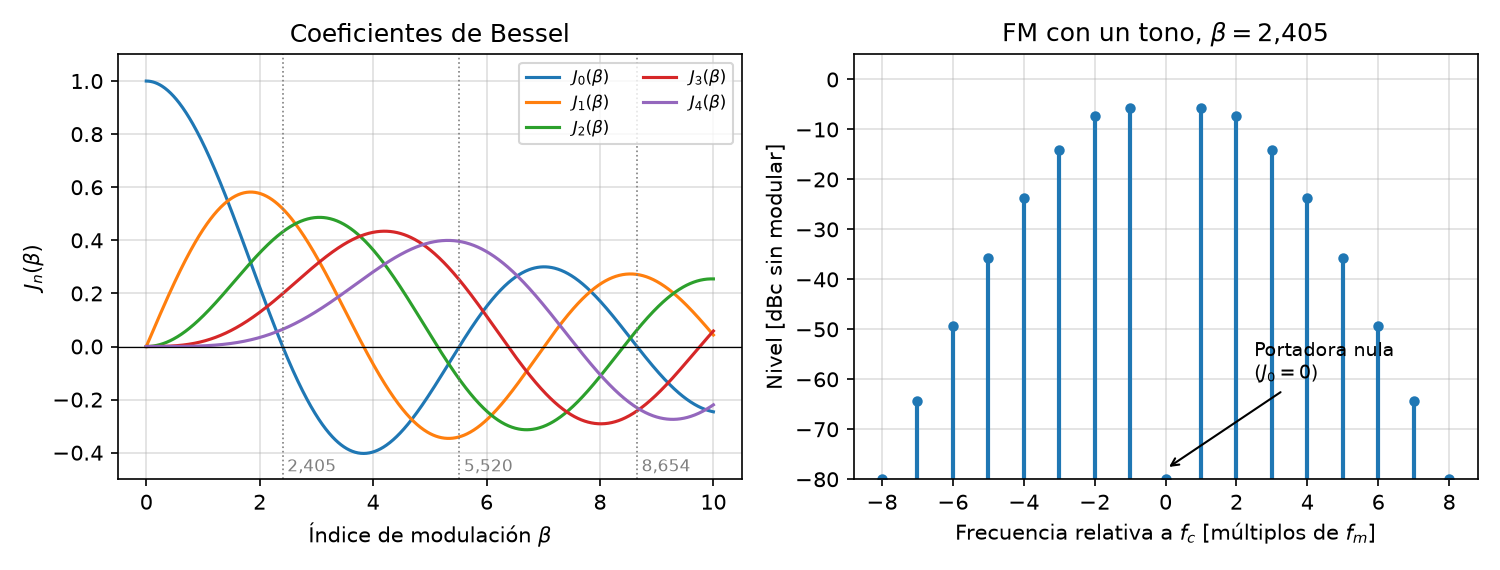
\includegraphics[width=\textwidth]{teoria/fm_bessel.png}
    \caption{Coeficientes de Bessel en función de $\beta$ y espectro de FM con portadora nula.}
    \label{fig:fm_bessel}
\end{figure}

Esta relación no permite medir el índice de modulación de una emisión de programa habitual, por tres razones:
\begin{itemize}
    \item La señal modulante es compleja: tiene muchas componentes de frecuencia y amplitud variables. El índice $\beta = \Delta f / f_m$ solo está definido para un tono, y con varios tonos aparecen productos de intermodulación con coeficientes $J_n(\beta_1) J_k(\beta_2) \cdots$.
    \item El espectro cambia continuamente con el contenido del programa, de modo que la línea de la portadora sube y baja todo el tiempo.
    \item La señal estéreo incluye, además del audio, el tono piloto, las bandas laterales de $S$ alrededor de $38 \, [kHz]$ y, si existe, el RDS, que también modulan la portadora.
\end{itemize}

\subsection{Síntesis}
La FM transmite la información en la frecuencia instantánea de la portadora, con amplitud constante. Esto la hace robusta frente al ruido y a las variaciones de amplitud del canal, y permite usar amplificadores no lineales. A cambio, ocupa un ancho de banda mucho mayor que la AM: unos $200 \, [kHz]$ contra $10 \, [kHz]$. En el analizador se ve como un bloque de energía de ancho variable alrededor de la frecuencia del canal, con potencia total constante y una distribución que cambia con el programa.

En la medición, la emisora de $88{,}9 \, [MHz]$ ocupó unos $220 \, [kHz]$ de ancho de banda, entre los valores de Carson para una emisión monofónica y una estéreo, y una emisora en el canal adyacente mostró que los flancos de canales contiguos llegan a acercarse hasta el piso de ruido.